\documentclass[twocolumn,a4paper]{article}
\usepackage[utf8]{inputenc}
\usepackage{listings}
\usepackage{titling}
\usepackage{booktabs}
\usepackage{hyperref}
\usepackage{tabularx}
\usepackage[]{footmisc}
\usepackage{gensymb}
\usepackage{float}
\usepackage[table,xcdraw]{xcolor}
\usepackage[skip=2pt]{caption}
\usepackage{amsmath}
\usepackage{graphicx}
\usepackage{matlab-prettifier}
\graphicspath{ {./images/} }

\newcommand{\subtitle}[1]{
  \posttitle{
    \par\end{center}
    \begin{center}\large#1\end{center}
    \vskip0.5em}
}

\lstset{style=Matlab-editor}
\title{Intelligent system for color difference recognition\\ in an industrial color copy process}
\subtitle{Intelligent Systems, Department of Information Engineering, University of Pisa}
\author{Federico Rossi}
\date{2017/2018}
\begin{document}

\maketitle
\section{Part I}
\subsection{Introduction}
In the first part of this work we'll need to:
\paragraph{Step 1}Generate reasonable noisy spectra from the master spectra, convert them into CIE $L^*a^*b^*$ format and, for now, compute the target differences between a master and the corespondent copy $\Delta E$ using the following formula (by means of \texttt{de(LAB1,LAB2)} function included in the \texttt{optprop} MATLAB library):
    \begin{equation}\label{eqn:formula}
        \Delta E^* = \sqrt{(L_1^*-L_2^*)^2+(a_1^*-a_2^*)^2+(b_1^*-b_2^*)^2}
    \end{equation}
\paragraph{Step 2}Take the output of the previous step - that is a matrix of dimension $[421*2; 1269*n]$ where $n$ is the number of copies we have generated for each master sample - and extract features from it (to reduce reasonably the number of \texttt{rows} into a set that best represents the original spectrum).
\paragraph{Step 3}Train a shallow neural network to solve a \textit{function fitting problem} with the previous sub-sampled spectra as inputs and the differences computed at step 1. as targets.
\subsection{Step 1 - Generation of copies}
To generate copies from a master patch we must introduce some kind of noise to the spectrum, in order to slightly change the final color.
\paragraph{} To generate a random, yet repeatable, noise the following snippet of code has been used in MATLAB:
\begin{lstlisting}
rng(12); %set the seed
for i=1:numcopies
    noise=random('unif',1,1.13);
    copy=spectra*noise;
end
\end{lstlisting}

Parameters of uniform distributions are chosen empirically to obtain a maximum difference of $5$.

At this point, if we convert the noisy spectrum back to the CIE $L^*a^*b^*$ format using \texttt{roo2lab} function from \texttt{optprop}, we can compute the target difference between the master patch and the copy patch using the \texttt{de} function.

\begin{figure}
    \centering
    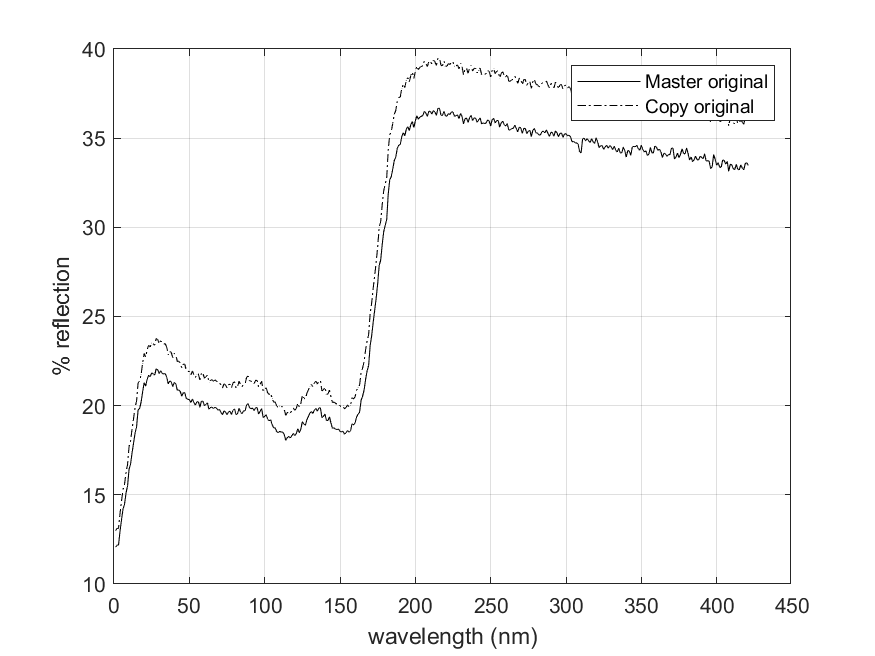
\includegraphics[scale=0.5]{images/C_5_120_masterCopy.png}
    \caption{Master spectrum compared to its copy spectrum}
    \label{fig:master_copy}
\end{figure}
\clearpage
\begin{figure}
    \centering
    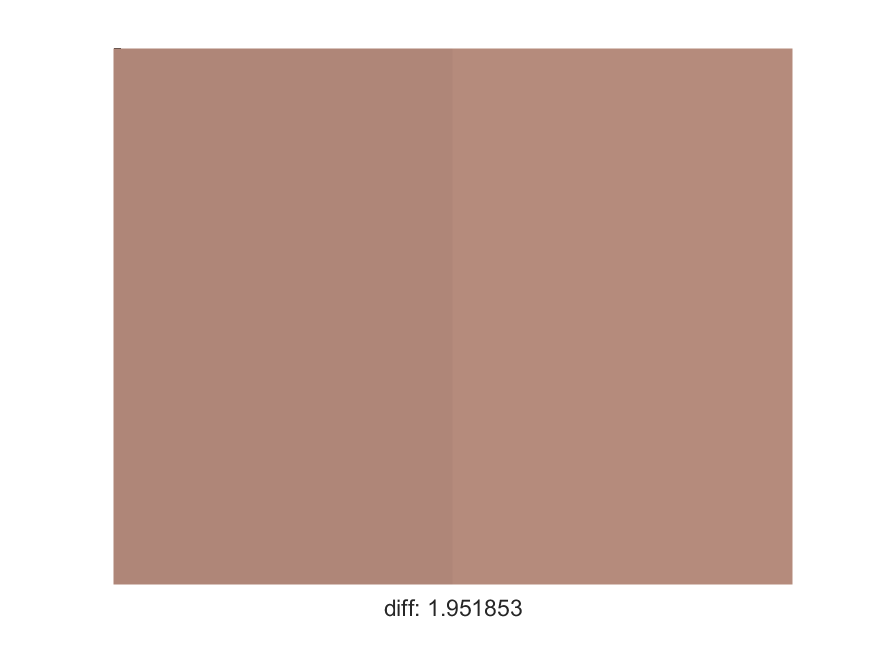
\includegraphics[scale=0.3]{images/E_120_masterCopyView.png}
    \caption{Master color compared to its copy}
    \label{fig:master_copy_col}
\end{figure}
\paragraph{Example} An example of a master spectrum and the noisy copy is shown in Figure \ref{fig:master_copy}. Figure \ref{fig:master_copy_col} shows the master color and its copy color. 
\paragraph{Output} Then the output of this step is composed as follow:
\begin{itemize}
    \item \texttt{masterCopyExpectedDiff} a $[1; 1269*n]$ matrix containing the target differences computed as before.
    \item \texttt{masterCopyPairs} a $[421*2; 1269*n]$ matrix containing, for each column, the pair:
    \begin{equation}
        <\text{master}[1,421]; \text{copy} [422,842]>
    \end{equation}
\end{itemize}
\subsection{Step 2 - Feature extraction and selection}
The output of the previous step is clearly too big in terms of a single sample to be feed to a shallow neural network. Therefore we need to reduce the quantity of information provided per sample, maintaining quite the same quality. 
\paragraph{} The idea is to divide the spectrum in $k$ wavelength ranges of size $M$, and internally aggregate the information. For our purposes, an aggregation function used is shown in Equation \ref{eqn:mov_avg}. Using this formula, as a side, we also manage to remove some noise from original data.
\begin{equation} \label{eqn:mov_avg}
	m_i = \frac{1}{M} \sum_{j=i-\frac{M}{2}}^{i+\frac{M}{2}} s_j,  i = \frac{(2l+1)*M}{2}, \forall l \in [0,\frac{S}{M}-1]
\end{equation}
Where $s_j$ is the original signal's sample, $m_i$ is the result of the aggregation window and $S$ is the number of original samples.
\paragraph{How to choose $k$} If $k$ is too small we are loosing too much information from the aggregation; on the other hand, if we sub-sample the spectrum with an high number of ranges we are not compressing the information enough. Figure \ref{fig:master_subsmplmul} shows how aggregation varies increasing $k$.
\paragraph{} Trying some different parameters for $k$, the ones that are a good trade-off between information compression and information loss are $k \in [5,20]$. From now on, we will go for the higher aggregation and see if performances are good enough.

Recalling the previous example, the aggregation result for $k=5$ is shown in \ref{fig:master_subsmpl}, thus obtaining $10$ features for each pair.
\begin{figure}
    \centering
    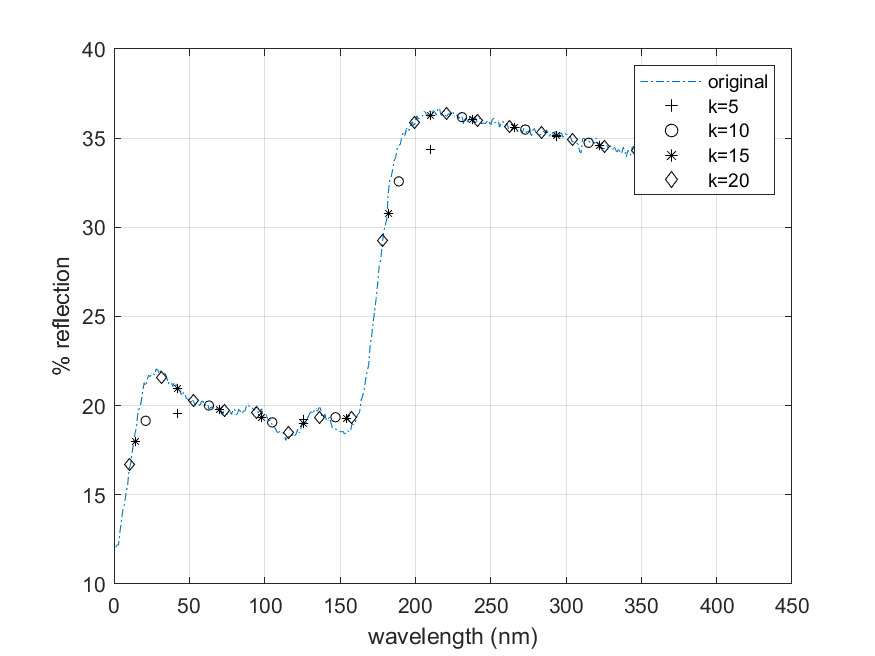
\includegraphics[width=\linewidth]{images/120_5_5_20_masterSub.png}
    \caption{Master spectrum compared to the various aggregate versions}
    \label{fig:master_subsmplmul}
\end{figure}

\begin{figure}
    \centering
    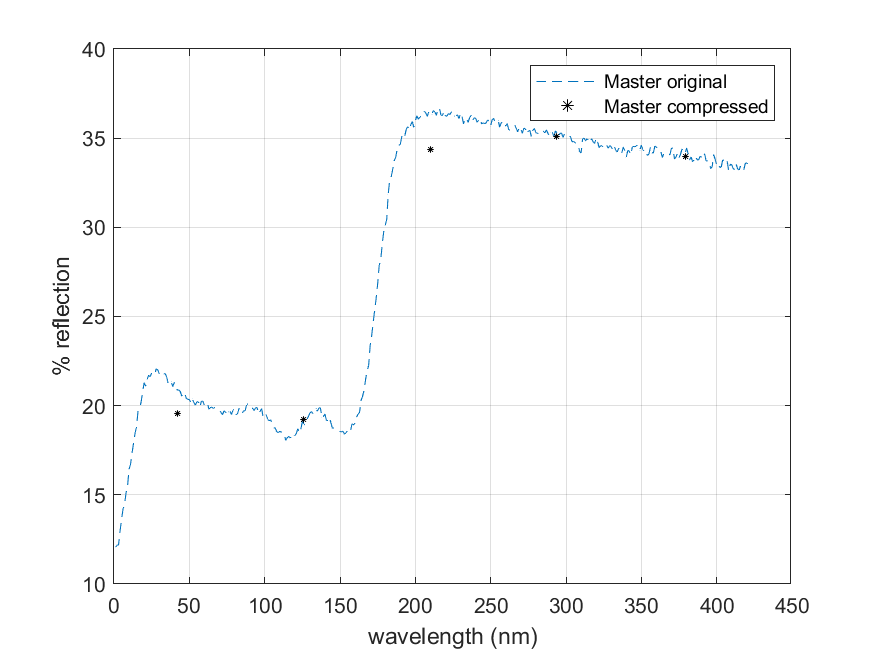
\includegraphics[width=\linewidth]{images/A_5_120_masterSub.png}
    \caption{Master spectrum compared to the aggregate version with k=5}
    \label{fig:master_subsmpl}
\end{figure}
\paragraph{Selection} We set up \texttt{sequentialfs} from MATLAB to extract the $4$ best features that approximate Formula \ref{eqn:formula}, using the \texttt{mse} from a fitting operation as choice criterion.
\paragraph{Output} The output from this step is:
\begin{itemize}
    \item \texttt{masterCopyPairsMean} a $[4; 1269*n]$ containing the selected features.
\end{itemize}
\subsection{Step 3 - Fitting network}\label{sec:nnet} Now that we have our \textit{inputs} and \textit{targets} we can feed them into a shallow neural network for function fitting. 
\paragraph{} We create the network in MATLAB using the \texttt{fitnet} function, with size of hidden layer equal to $n$:
\begin{lstlisting}
hiddenLayerSize=n
net=fitnet(hiddenLayerSize);
net.divideParam.trainRatio=70/100;
net.divideParam.valRatio=15/100;
net.divideParam.testRatio=15/100;
net=train(net,inputs,targets);
\end{lstlisting}
\begin{figure}
    \centering
    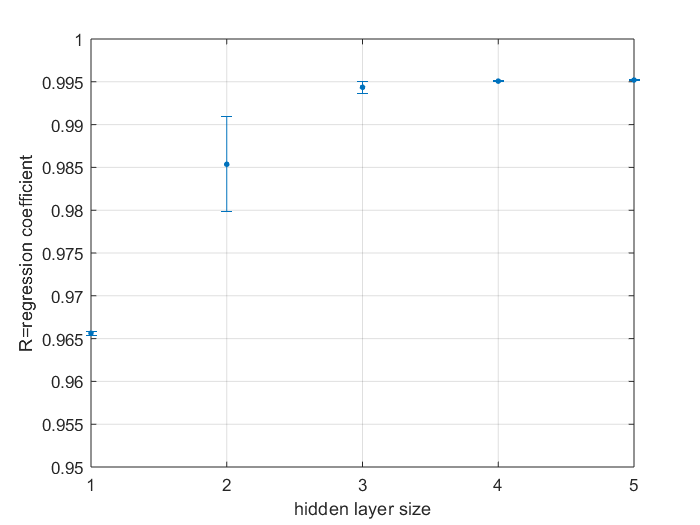
\includegraphics[width=\linewidth]{images/r_perf_ci.png}
    \caption{Values of R vs number of neurons}
    \label{fig:r_vs_num_neur}
\end{figure}

\paragraph{Performance} At the end of the training phase, we measure the performances of the neural network in terms of \textit{mean squared error} and \textit{regression coefficient}. 
\paragraph{Evaluation} Performance evaluation consists in repeating the training a certain number of times ($10$ in our case, since performance metrics are not too jittery). 

The randomness of different repetitions is introduced by the \texttt{dividerand} option used by MATLAB to subdivide the provide dataset into \textit{training},\textit{validation} and \textit{testing} folds.
\paragraph{How to choose n} High values of $n$ will require more training samples and time but, at the same time, will produce more accurate results in terms of \textit{regression coefficient}.
Lower values will visibly reduce the amount of time and samples required to train the network but will produce less accurate results. Figure \ref{fig:r_vs_num_neur} shows the behavior of R compared to number of neuron in hidden layer (values reported are the average of $10$ repetitions with a $95\%$ confidence interval).
\paragraph{Training profiling} Moreover profiling the training script with the MATLAB tool produced results in Table \ref{tab:prof_res}.
\begin{table}[]
\centering
\begin{tabular}{|c|c|}
\hline
\textbf{Hidden layer size} & \textbf{Execution time (s)} \\ \hline
1                          & $1 \pm 0$                           \\ \hline
2                          & $2 \pm 0.1$                           \\ \hline
3                          & $3 \pm 0.2$                           \\ \hline
4                          & $3.2 \pm 0.2$                          \\ \hline
5                          & $3.4 \pm 0.3$                         \\ \hline
\end{tabular}
\caption{Profiling results from MATLAB profile tool (10 reps, $95\%$ CI)}
\label{tab:prof_res}
\end{table}
\begin{figure}
	\centering
	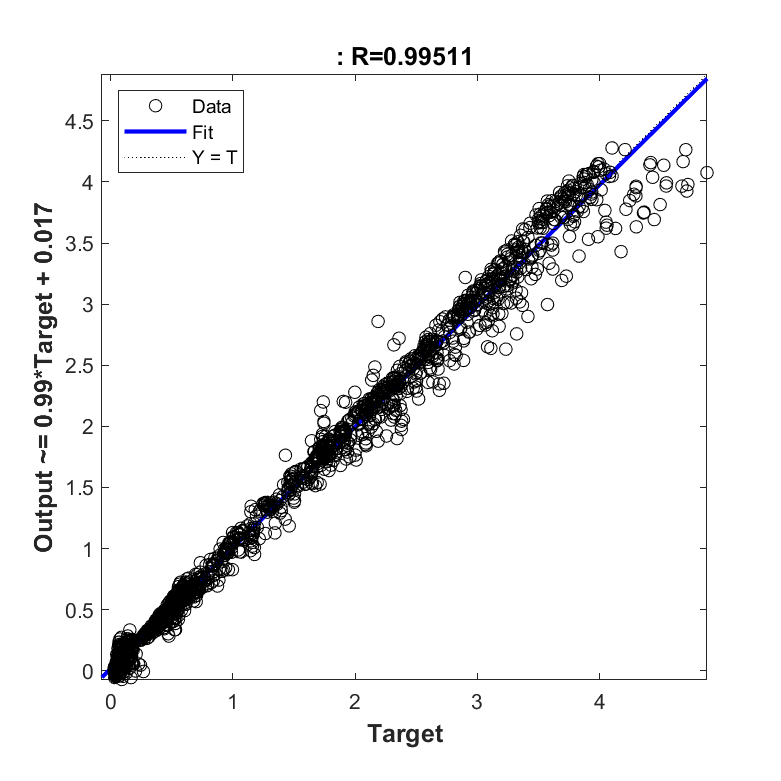
\includegraphics[width=\linewidth]{images/net_4_reg.png}
	\caption{Regression plot}
	\label{fig:r_plot}
\end{figure}
\paragraph{} So, from previous considerations, the choice of $4$ hidden neurons in the hidden layer of the network is a good trade-off between network performances and training time.
Results are the following (considered $95\%$ confidence interval):
\begin{equation}\label{eqn:regression}
    \text{regression} = 0.995076 \pm 0.000057
\end{equation}
\begin{equation}
    \text{mse} = 0.016 \pm 0.0001
\end{equation}

Figure \ref{fig:r_plot} shows one repetition's regression plot.
\paragraph{} As we can see from Equation \ref{eqn:regression}, the regression coefficient is very close to $1$, thus the fitting is good.
\paragraph{Note}The \textit{mse}'s order of magnitude must be compared to a meaningful granularity from the target sets, that in our case is around $0.1$.
\clearpage
\section{Part II}
In the second part we need to take into account some imprecisions that might occur in Equation \ref{eqn:formula}. 
We'll make use of another color space, called CIE $L^{*}c^{*}h^{*}$ - that, in this case, is a cylindric coordinates system.

In particular, in the second part, we'll need to:
\begin{itemize}
	\item Find out the areas of the CIE $L^*a^*b^*$ sphere that lead to imprecisions in the formula w.r.t an external observer.
	\item Express those areas by means of a set of \textit{fuzzy rules} on \textit{fuzzy input sets} that we'll explain later on.
	\item Adjust the output of Equation \ref{eqn:formula} using a \textit{fuzzy system} that works on previous defined \textit{fuzzy rules} and use the new adjusted values as the \textit{targets} of the neural network built in Sub-section \ref{sec:nnet}.
\end{itemize}
\subsection{Step 1 - $\mathbf{\Delta E}$ imprecisions}\label{subsec:imprec}
\begin{figure}[H]
	\centering
	
\includegraphics[scale=0.5]{images/darkred_darkblue.png}
	\caption{Dark red and dark blue patches}
	\label{fig:darkredblue}
\end{figure}
\begin{figure*}
	\centering
	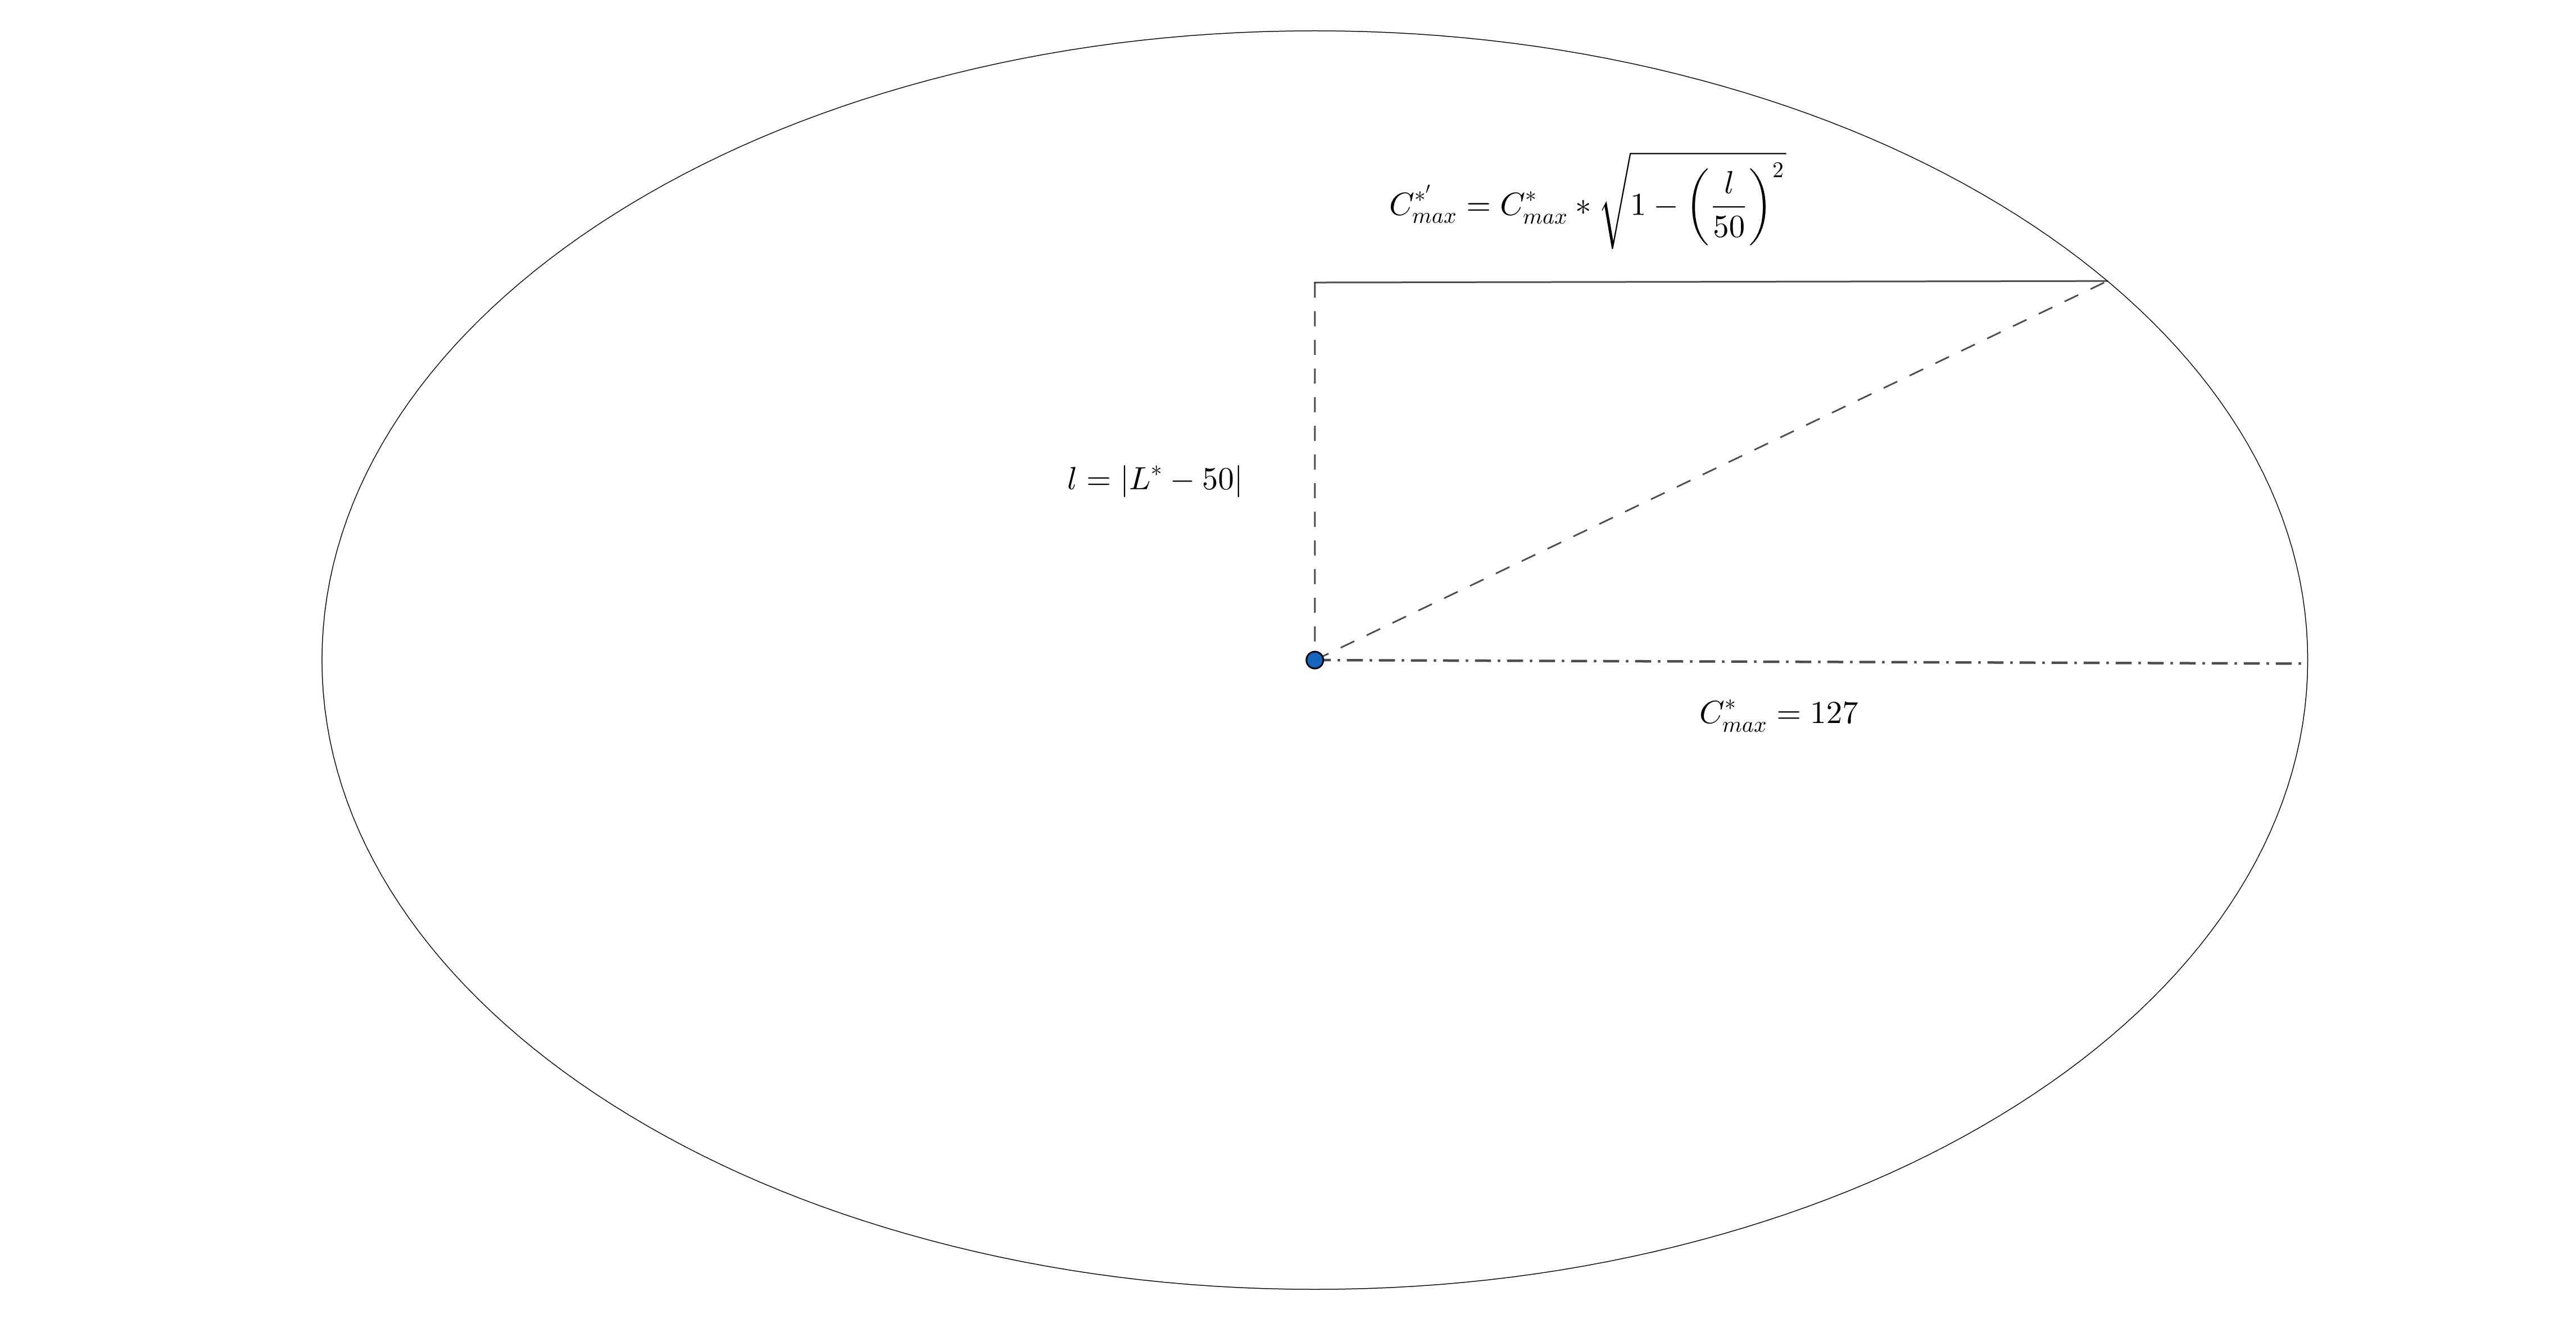
\includegraphics[width=\linewidth]{images/ellipsis.png}
	\caption{$L^*c^*h^*$ sphere approximation}
	\label{fig:sphere_approx}
\end{figure*}
\paragraph{Dark colors} First set of imprecisions occurs when we have colors which are very dark. For example, in Figure \ref{fig:darkredblue} are reported, respectively, a dark red patch and a dark blue one. If we use \ref{eqn:formula} to compute color difference we get $\Delta E^{*} \sim 10$ but, if we apply the definition for color difference from CIE, that pair of colors should have a difference between $0$ and $1.5$, so the output of the formula must be adjusted in this direction.\footnote{Project specifications}
\paragraph{The blue-violet area} In this area the reported $\Delta E^*$ is typically smaller than perceived difference, so we could think of increasing its value.\footnote{\label{note:opentext} https://opentextbc.ca/graphicdesign/chapter/4-4-lab-colour-space-and-delta-e-measurements/}.
\paragraph{The yellow area} In this area instead we experience the opposite behavior - that is, the perceived difference is typically smaller than the one reported by $\Delta E^*$ (also in Note \ref{note:opentext}).
\paragraph{Unsaturated colors} Another area is defined by colors that are unsaturated and not too much dark. Here the formula will compress our perceived difference, so we'll need to adjust it by increments.
\subsection{Step 2 - Fuzzy sets and rules}
\subsubsection{Fuzzy sets} We want to model a \textit{linguistic variable} for each L,c,h and original $\Delta E^{*}$ \textit{crisp set} that represents concepts exploited in defining imprecision areas in Sub-section \ref{subsec:imprec}. Membership functions for sets are shown is following figures:
\begin{itemize}
	\item \textit{Luminosity} figure \ref{fig:mfl}. Range is $[0,100]$ according to CIE standards.
	\item \textit{Hue} figure \ref{fig:mfh}. Range is $[0\degree ,360\degree]$ according to CIE standards.
	\item \textit{Chroma} figure \ref{fig:mfc}. Chroma range depends on $L^*$ value, and it is known to span from $0$ to $C^{*}_{max} = 127$ at $L^*=50$.
	So the maximum saturation may happen slightly before that value for values of $L^*$ far from $50$. So we may think to approximate the the relation between $L^*$ and $C^*$ as an ellipsis shape: \[ \frac{c^{*2}}{C^{*2}_{max}}+\frac{l^2}{50^2} = 1  \] (where $l = \left | L^* -50 \right |$). Then we compute the $C^{*'}_{max}$ as in Figure \ref{fig:sphere_approx}. Then we scale the $c^*$ value as \[c^{*}_{\%} = 100*\frac{c^*}{C^{*'}_{max}}\]
	Where $C^{*}_{max} = 127$. Therefore, the range we assume for $c^{*}$ is $[0,100]$.
	\item \textit{Original $\Delta E^{*}$} figure~\ref{fig:mfde}. Range is $[0,8]$ according both to project specifications and empirical outcomes.
\end{itemize}

\subsubsection{Fuzzy rules} According to considerations in Sub-section \ref{subsec:imprec},some of the rules inserted into the \textit{rule base} are shown in Table \ref{tab:rules}
\begin{table*}[]
\centering
\rowcolors{2}{gray!25}{white}
\begin{tabular}{|c c c c c |}
\hline
\rowcolor{gray!50}
L & c  & h & $\Delta E^*_{orig}$ & $\Delta E^*_{adj}$ \\ \hline
dark       & -           & -          & -                 & no\_diff              \\ \hline
not dark   & saturated   & yellow     & unexpdiff         & expdiff               \\ \hline
not dark   & saturated   & yellow     & cleardiff         & unexpdiff             \\ \hline
not dark   & saturated   & blue       & expdiff           & unexpdiff             \\ \hline
not dark   & saturated   & blue       & unexpdiff         & cleardiff             \\ \hline
not dark   & saturated   & violet     & expdiff           & unexpdiff             \\ \hline
not dark   & saturated   & violet     & unexpdiff         & cleardiff             \\ \hline
not dark   & unsaturated & -          & expdiff           & unexpdiff             \\ \hline
not dark   & unsaturated & -          & unexpdiff         & cleardiff             \\ \hline
\end{tabular}
\caption{Main rules applied in the mamdani fuzzy inference system}
\label{tab:rules}
\end{table*}
\begin{figure}
	\centering
	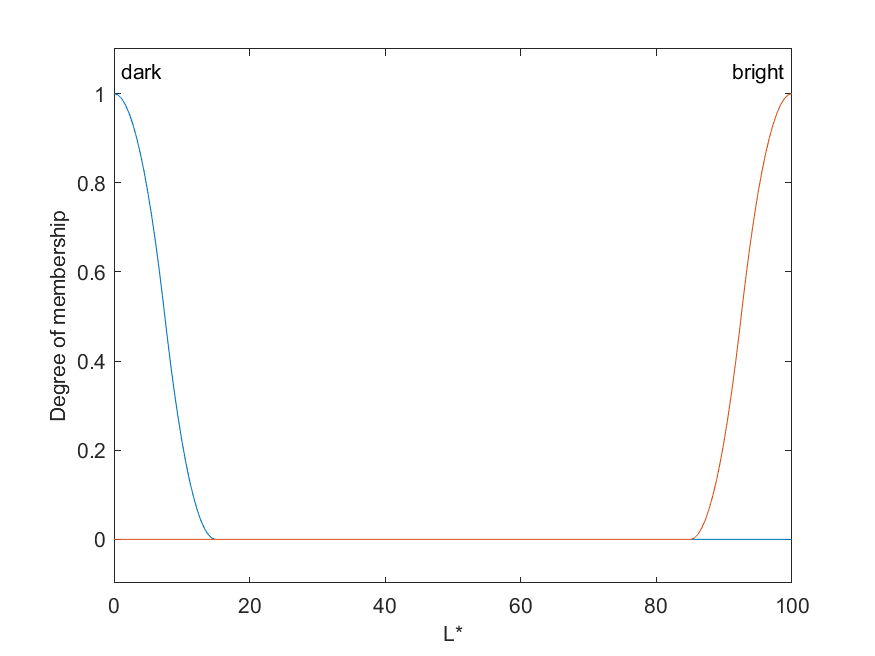
\includegraphics[scale=0.5]{images/mf_L.png}
	\caption{Luminosity membership function}
	\label{fig:mfl}
\end{figure}
\begin{figure}
	\centering
	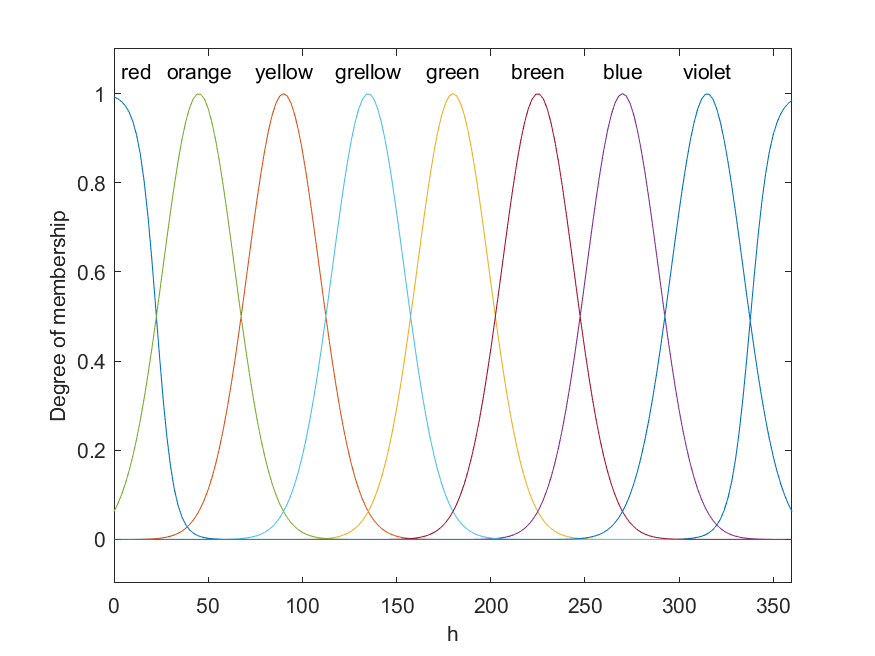
\includegraphics[scale=0.5]{images/mf_h.png}
	\caption{Hue membership function}
	\label{fig:mfh}
\end{figure}
\begin{figure}
	\centering
	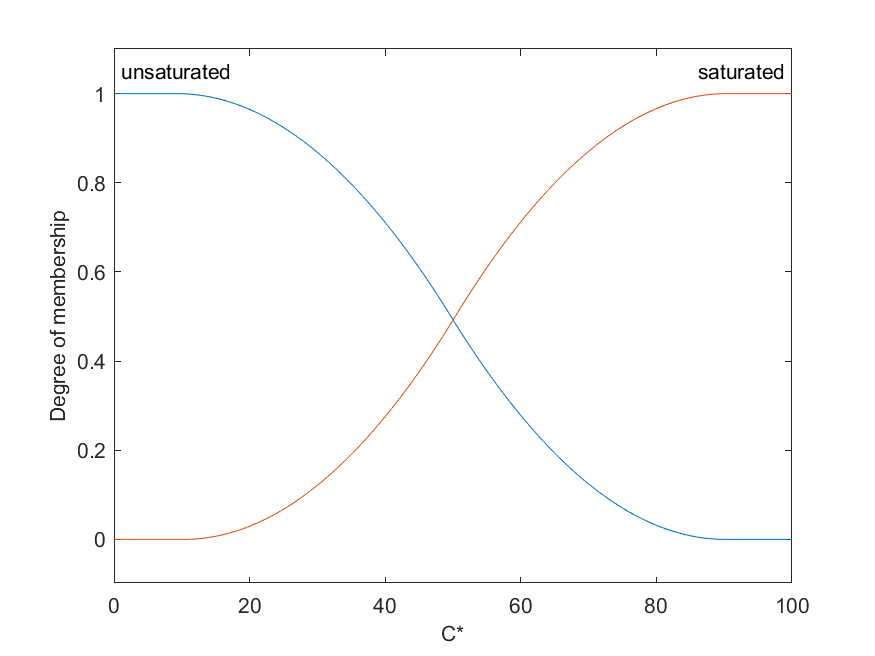
\includegraphics[scale=0.5]{images/mf_c.png}
	\caption{Chroma membership function}
	\label{fig:mfc}
\end{figure}
\begin{figure}
	\centering
	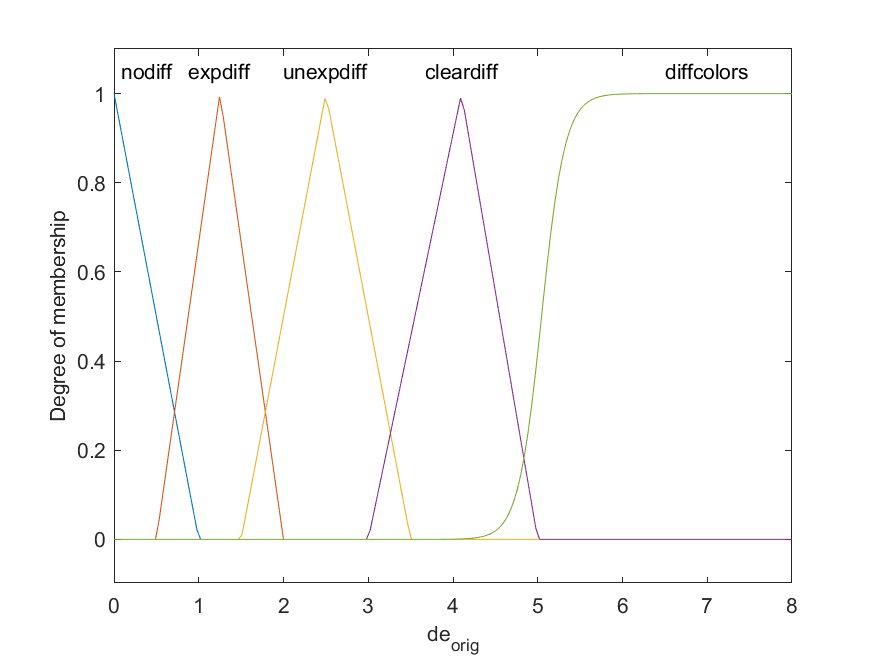
\includegraphics[scale=0.5]{images/mf_de.png}
	\caption{$\Delta E^{*}$ membership function both for input and output}
	\label{fig:mfde}
\end{figure}
\clearpage
\subsection{Step III - Fitting network with new data} At this point of the work we have again inputs represented by pairs of masters and copies and targets represented  by corrected $\Delta E^*_{adj}$. We submit these data to the network defined in Sub-section \ref{sec:nnet} for training.

Performance metrics over 10 repetitions are:
\begin{equation}
	R=0.984801 \pm 0.002223
\end{equation}
\begin{equation}
\text{mse} = 0.051570 \pm 0.007305
\end{equation}
\paragraph{NOTE} We can obtain a regression coefficient similar to the first part of the project is we reasonably increase the number of neurons ($\sim 50$) and as a consequence, the time required to train the network. Therefore we obtain, on $10$ repetitions of training these testing performances, that are quite comparable to the ones obtained in the first part, but now with differences recognized closer to the perceived ones. 
\begin{equation}
	R=0.993290 \pm 0.001360
\end{equation}
\begin{equation}
	\text{mse} = 0.018770 \pm 0.003756
\end{equation}
\section{Conclusion and examples} At the end we apply the whole system to a pair of selected master and copy patches (not provided during training phase), one belonging to the violet area,one belonging to the unsaturated area and one belonging to the yellow area\\
Figure \ref{fig:violet_example} shows how the original difference was too way different from the perceived one, reporting quite no differences between the two samples while having a visible difference.\\
Figure \ref{fig:unsaturated_example} shows the same concept but with saturated colors. Note that this pair of samples behaves in different ways according to the view angle. However, for sure, the perceived difference is not the one reported by the original formula.\\
Figure \ref{fig:yellows_example} shows the opposite concept applied to the yellow area. As we can see, the reported difference was too higher for that pairs of colors, reporting two completely different colors instead of a clear difference between them.
\newpage
\begin{figure}[H]
	\centering
	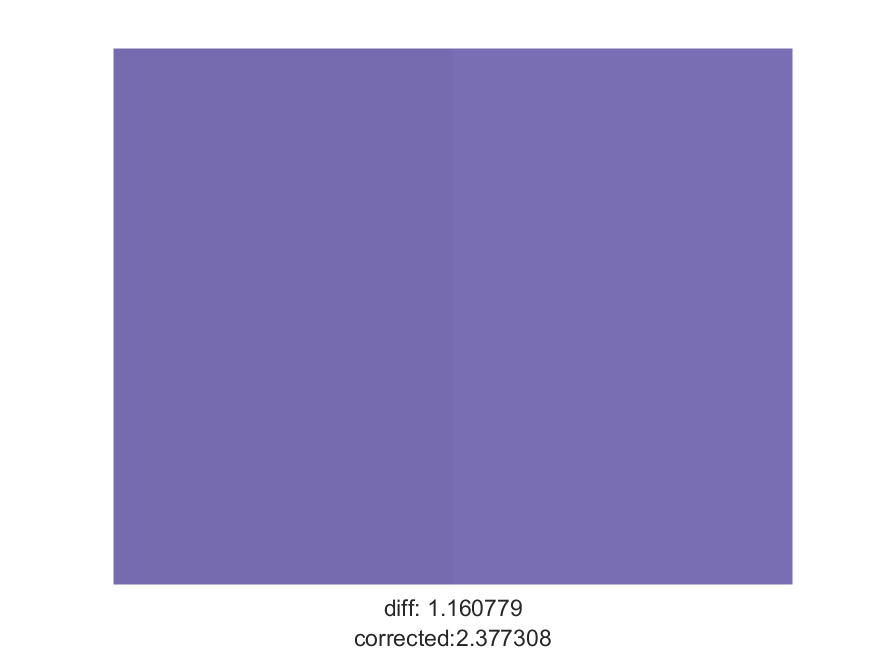
\includegraphics[scale=0.5]{images/example_violet.png}
	\caption{Violet area difference and correction}
	\label{fig:violet_example}
\end{figure}

\begin{figure}[H]
	\centering
	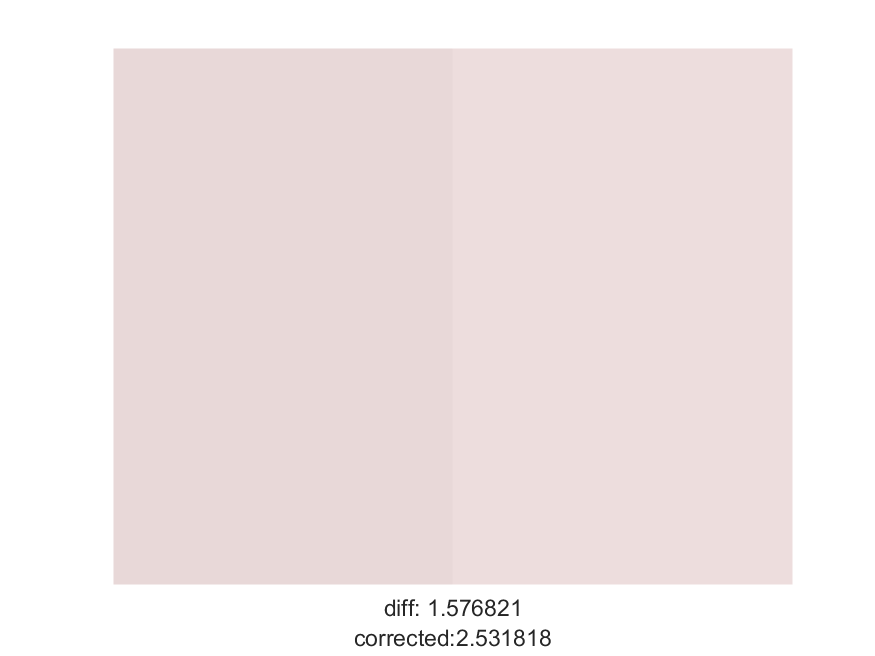
\includegraphics[scale=0.5]{images/example_unsaturated_2.png}
	\caption{Unsaturated area difference and correction}
	\label{fig:unsaturated_example}
\end{figure}

\begin{figure}[H]
	\centering
	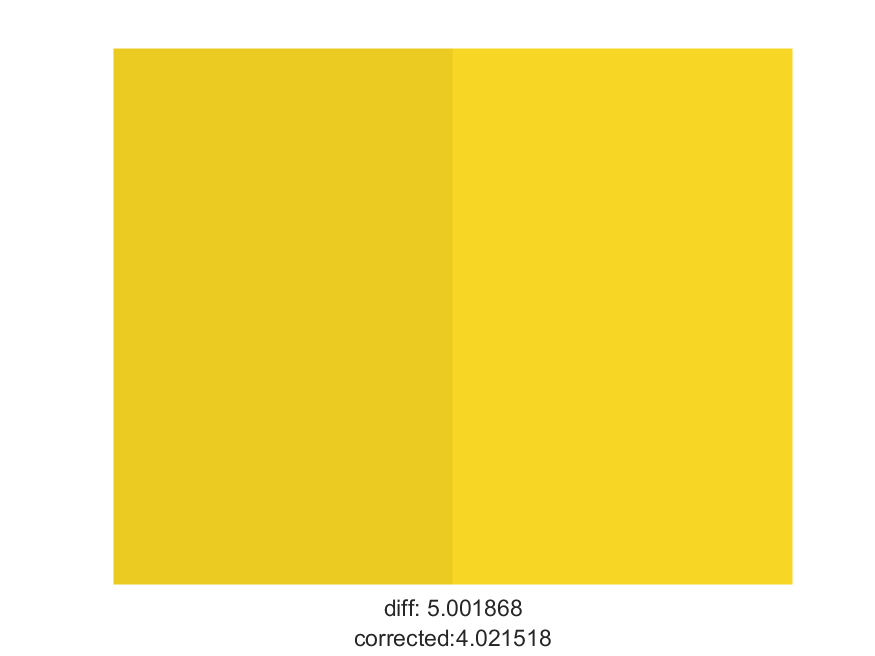
\includegraphics[scale=0.5]{images/example_yellows.png}
	\caption{Yellow area difference and correction}
	\label{fig:yellows_example}
\end{figure}
\end{document}
